\documentclass[10pt]{article}
\usepackage{fullpage}
\usepackage{amsmath}
\usepackage[amsthm, thmmarks]{ntheorem}
\usepackage{amssymb}
\usepackage{graphicx}
\usepackage{enumerate}
\usepackage{verse}
\usepackage{tikz}
\usepackage{verbatim}
\usepackage{hyperref}

\newtheorem{lemma}{Lemma}
\newtheorem{theorem}[lemma]{Theorem}
\newtheorem{definition}[lemma]{Definition}
\newtheorem{proposition}[lemma]{Proposition}
\newtheorem{corollary}[lemma]{Corollary}
\newtheorem{claim}[lemma]{Claim}
\newtheorem{example}[lemma]{Example}

\newcommand{\dee}{\mathrm{d}}
\newcommand{\Dee}{\mathrm{D}}
\newcommand{\In}{\mathrm{in}}
\newcommand{\Out}{\mathrm{out}}
\newcommand{\pdf}{\mathrm{pdf}}
\newcommand{\Cov}{\mathrm{Cov}}
\newcommand{\Var}{\mathrm{Var}}

\newcommand{\ve}[1]{\mathbf{#1}}
\newcommand{\mrm}[1]{\mathrm{#1}}
\newcommand{\etal}{{et~al.}}
\newcommand{\sphere}{\mathbb{S}^2}
\newcommand{\modeint}{\mathcal{M}}
\newcommand{\azimint}{\mathcal{N}}
\newcommand{\ra}{\rightarrow}
\newcommand{\mcal}[1]{\mathcal{#1}}
\newcommand{\X}{\mathcal{X}}
\newcommand{\Y}{\mathcal{Y}}
\newcommand{\Z}{\mathcal{Z}}
\newcommand{\x}{\mathbf{x}}
\newcommand{\y}{\mathbf{y}}
\newcommand{\z}{\mathbf{z}}
\newcommand{\tr}{\mathrm{tr}}
\newcommand{\sgn}{\mathrm{sgn}}
\newcommand{\diag}{\mathrm{diag}}
\newcommand{\Real}{\mathbb{R}}
\newcommand{\sseq}{\subseteq}
\newcommand{\ov}[1]{\overline{#1}}

\DeclareMathOperator*{\argmin}{arg\,min}

\title{Gradient-Domain Path Tracing}
\author{Pramook Khungurn}

\begin{document}
  \maketitle

  This document is written as I read the ``Gradient-Domain Path Tracing'' paper \cite{Kettunen:2015}.

  \section{Introduction}

  \begin{itemize}
  	\item There has been recent works that extends Metropolis light transport to compute gradients of the resulting image instead of computing the pixel colors.

  	\item This paper shows that you can do that in normal path tracing as well.  
  	\begin{itemize}
  		\item Instead of tracing a single path, shoot an additional finite-difference path shifted by one pixel.  This gives you image contribution of each path and also an estimate of the finite difference between the two pixels.

  		\item In the end, perform a screened Poisson reconstruction that combines all information: both the image contributions and the gradient estimate.
  	\end{itemize}

  	\item The gradient is not estimated from difference of two uncorrelated random paths.  The paths generated are highly correlated, and this lowers the variance.

  	\item Gradient rendering yields better quality than direct value rendering when the resuling image has less energy in high frequencies than in low frequencies.  The screend Poisson reconstruction can get the best of both worlds.  	

  	\item The paper introduce new sampling strategies:
  	\begin{itemize}
  		\item A new shift mapping whose Jacobian is very easy to calculate.
  		\item The gradient can either be approximated with forward or inverse shift.  These can be combined with multiple importance sampling to yield better results.
  	\end{itemize}

  	\item As a note, the screen Poisson reconstruction takes as input the gradient image $I^{\dee x}$ and $I^{\dee y}$ and a rough estimate of the actual image $I^g$.  It solves for the image $I$ by solving the following minimization problem:
  	\begin{align*}
  		\argmin_I \bigg( \left\| \begin{pmatrix}
  			H^{\dee x} I \\ H^{\dee y} I \\ 
  		\end{pmatrix} - \begin{pmatrix}
  			I^{\dee x} \\
  			I^{\dee y}
  		\end{pmatrix} \right\|^2_2 
  		+ \| \alpha (I - I^g) \|^2_2 \bigg)
  	\end{align*}
  	where $H^{\dee x}$, $H^{\dee y}$ are matrices that take finite differences along both rows and columns and returns appropriately vectorized gradients, and $\alpha$ is a weighting parameter.
  \end{itemize}

  \section{Overview}

  \begin{itemize}
  	\item Image gradient $=$ differences between pairs of neighbor pixels.

  	\item Gradient-domain rendering samples image gradients instead of pixel values.

  	\item In gradient-domain path tracing, each \emph{base path} is paired with an \emph{offset path} through the neighboring pixel.  See the picture below for what they look like.
  	\begin{center}
  		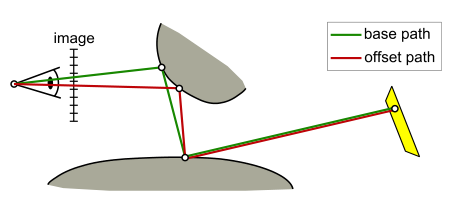
\includegraphics[width=4in]{base-offset.png}
  	\end{center}

  	\item The \emph{shift mapping} computes the offset path from the base path.

  	\item The difference between the contribution of the two paths gives an estimate of the gradient.

  	\item More precisely, let $\Delta_{i,j}$ denote the difference between pixels $i$'s and $j$'s contribution:
  	\begin{align*}
  		\Delta_{i,j} = \bigg( h(x) * \int_{\Omega} f(x, \bar p)\ \dee\mu(\bar p) \bigg)(x_i) - 
  		\bigg( h(x) * \int_{\Omega} f(x, \bar p)\ \dee\mu(\bar p) \bigg)(x_j)
  	\end{align*}
  	where:
  	\begin{itemize}
  		\item $x$ is the image coordinate,
  		\item $h(x)$ is the pixel filter,
  		\item $\Omega$ is the space of all light paths,
  		\item $(x, \bar p)$ is the path where $\bar p$ denotes all the path configurations from a point on the sensor to a light source,
  		\item $f$ is the image contribution function.
  	\end{itemize}
  	The pixel filters are evaluated at pixel centers $x_i$ and $x_j$.

  	\item The above definition of $\Delta_{i,j}$ are what was used in previous works on gradient-domain rendering.  The paper, however, tries to estimate the difference with a single integral:
  	\begin{align*}
  		\Delta_{i,j} 
  		= \bigg( h(x) * \int_{\Omega} f(x, \bar p) - f(T_{ij}(x, \bar p)) |T'_{ij}|\ d\mu(\bar p) \bigg)
  		= \bigg( h(x) * \int_{\Omega} g_{ij}(x, \bar p)\ d\mu(\bar p) \bigg)
  	\end{align*}
  	where $T_ij$ is the shift mapping that deterministically maps a base path $(x,\bar p)$ to an offset path $T_{ij}(x, \bar p)$ such that they are close to each other in path space.  (The difference is only at the intersection?)

  	\item The $T_{ij}$ function only allows shifting by one pixel distance so that the filter value at the offset path is the same as that of the base path.  In this way, a single convolution is enough to define the gradient.
  \end{itemize}

  \section{Theoretical Analysis}

  \subsection{Error Analysis of Gradient Estimate}

  \begin{itemize}
  	\item To enable Fourier analysis, the paper makes the following assumptions:
  	\begin{itemize}
  		\item The image is 1D.
  		\item Paths are parameterized over a Cartesian hypercube, like the one used in Kelemen-style Metropolis light transport.
  		\item The first path dimension is the image axis.
  		\item All terms related to measure in path space are hided.
  		\item Analysis is only restricted to uniform sampling in the path space parameterization.  (No importance sampling is allowed?)
  		\item Sampling is statinary stochastic processes.  Basically, it means that it extends over an infinite domain, which implies that there is no boundaries to worry about.  This, however, tends to overestimate the variance of the real case in which the domain is finite.  	
  	\end{itemize}

  	\item The image contribution function $f$ is defined over an image axis $x$ and an orbitrary long vector of path parameters $\bar p$ (assumed to be the Cartesian hypercube like in Kelemen-style Metropolis light transport).

  	\item The shift mapping $T$ is given by $T(x, \bar p) = T(x-1, \bar p)$, which has unit gradient.

  	\item The path difference function $g$ is simply $g(x, \bar p) = f(x, \bar p) - f(x-1, \bar p)$, which can be written as the convolution $g(x, \bar p) = (d * f)(x, \bar p)$ where $d(x, \bar p) = \delta(x) - \delta(x-1).$ 

  	\item In Fourier domain, $g = d * f$ becomes $G = DF$.  The power spectrum of the path different function is given by:
  	\begin{align*}
  		|G(\omega_x, \omega_{\bar p})|^2 
  		&= |D(\omega_x, \omega_{\bar p})|^2 |F(\omega_x, \omega_{\bar p})|^2 \\
  		&= (2 - 2 cos(2\pi \omega_x)) |F(\omega_x, \omega_{\bar p})|^2 
  	\end{align*}
  	where $\omega_x$ and $\omega_p$ are frequencies over the image and path space.

  	\item We can observe from the above equation some well-known results:
  	\begin{itemize}
  		\item Finite difference cancels the DC.  This is because $|D(0, \omega_{\bar p})|^2 = 0$.
  		\item Finite difference attenuates low frequencies because $|D(\omega_x, \omega_{\bar p})|^2$ is low when $\omega_x$ is low.
  		\item Finite difference boosts square magnitudes of high frequencies by a factor up to four for the Nyquist limit $\omega_x = 1/2$ of the image.  This is because $|D(1/2, \omega_{\bar p})|^2 = 4$.
  	\end{itemize}

  	\item Given that the sampling gives rise to unbiased estimates, the variance is characterized by the mean square error (MSE).

  	\item Under a number of assumption, the expected squared errors in frequency domain $|\epsilon_F(\omega_x, \omega_{\bar p})|^2$ and $|\epsilon_G(\omega_x, \omega_{\bar p})|^2$ for all frequencies are constant:
  	\begin{align*}
  		|\epsilon_F(\omega_x, \omega_{\bar p})|^2 &= \frac{1}{n} \| F \|^2 \\
  		|\epsilon_G(\omega_x, \omega_{\bar p})|^2 &= \frac{1}{n} \| G \|^2 \\
  	\end{align*}
  	where
  	\begin{align*}
  		\| F \|^2 &= \int  |F(\omega_x, \omega_{\bar p})|^2\ \dee\omega_x \dee\omega_{\bar p} \\
  		\| G \|^2 &= \int  |G(\omega_x, \omega_{\bar p})|^2\ \dee\omega_x \dee\omega_{\bar p} 
  		= \int  (2 - 2\cos(2\pi\omega_x))|F(\omega_x, \omega_{\bar p})|^2\ \dee\omega_x \dee\omega_{\bar p} 
  	\end{align*}

  	\item Further analysis gives the MSE in the image domain only (by slicing the frequency domain at $\omega_{\bar p} = 0$).  Assuming perfect reconstruction kernel $h$, we have:
  	\begin{align*}
  		|\epsilon_F(\omega_x)|^2 = |\epsilon_F(\omega_x,0)|^2 = \frac{1}{n} \| F \|^2,\mbox{ if $|\omega_x| < 1/2$, otherwise 0,} \\
  		|\epsilon_G(\omega_x)|^2 = |\epsilon_G(\omega_x,0)|^2 = \frac{1}{n} \| G \|^2,\mbox{ if $|\omega_x| < 1/2$, otherwise 0,}
  	\end{align*}
  	which agrees with the behavior of standard Monte Carlo estimate.  	
  \end{itemize}

  \subsection{Analysis of Screened Poisson Reconstruction}
  \begin{itemize}
  	\item The MSE (variance) of the final image after screen Poisson reconstruction is given by:
  	\begin{align*}
  		|\epsilon_{R_\alpha}|^2 = \frac{1}{n} \frac{\alpha^4 \| F \|^2 + |D(\omega_x)|^2 \| G \|^2}{(\alpha^2 + |D(\omega_x)|)^2}.
  	\end{align*}

  	\item Using the above expression, if we set $\alpha = 0$ (i.e., using only gradient information), we have that
  	\begin{align*}
  		|\epsilon_{R_0}|^2 
  		= \frac{1}{n} \frac{|D(\omega_x)|^2 \| G \|^2}{(|D(\omega_x)|^2)^2}
  		= \frac{1}{n} \frac{ \| G \|^2}{|D(\omega_x)|^2}
  		= \frac{1}{n} \frac{ \| G \|^2}{2 - 2\cos(2\pi\omega_x)}.
  	\end{align*}
  	This implies that the gradient construction has a singularity at $\omega_x = 0$ (the DC).  However, when $\omega_x$ is high ($\omega_x = 1/2$ for example), then the variance reduces by a factor of $4$.  Thus, gradients are most benefitial at high frequencies.

  	\item The optimal value of $\alpha$ is given by $\alpha^2_*(\omega_x) = \| G \|^2 / \| F \|^2$, which gives the MSE of:
  	\begin{align*}
  		|\epsilon_{R_{\alpha_x}}|^2 = \frac{1}{n} \frac{\| G \|^2 \| F \|^2}{\| F \|^2 |D(\omega_x)|^2 + \| G \|^2}.
  	\end{align*}
  	The MSE approaches $\| F \|^2 /n $ at low frequency.  At high frequency ($\omega_x = 1/2$), the error becomes:
  	\begin{align*}
  		\frac{1}{n} \frac{\| G\|^2 \| F \|^2}{4 \| F \|^2  + \| G \|^2}
  		= \frac{1}{n} \frac{\| F \|^2}{4 \| F \|^2 / \| G \|^2  + 1}
  		\leq \frac{1}{n} \frac{\| F \|^2}{4 \| F \|^2 / \| G \|^2}
  		= \frac{1}{n} \frac{\| G \|^2}{4}.
  	\end{align*}
  	So, it is better than the full gradient reconstruction in this case.  Thus, if $4\| G\|^2 < \| F \|^2$, then the Poisson reconstruction is better than both.
  \end{itemize}

  \section{Gradient-Domain Path Tracing}
  
  The algorithm has already been outlined in previous sections.  This section talks about the implementation details.  	
  
  \subsection{Symmetric Gradients}
  
  \begin{itemize}
  	\item The gradient estimate is only valid if the shift mapping is a bijection of the path space onto itself, but it is hard to find such a mapping.

  	\item To dispense with the above requirement, they use the symmetric gradient formulation discussed in \cite{Manzi:2014}.

  	\item The symmetric gradient formulation works by computing the gradient with two integrals instead of one integral:
  	\begin{align*}
  		\Delta_{i,j} = \bigg( h(x) * \int_\Omega w_{ij}(x, \bar p) g_{ij}(x, \bar p)\ \dee\mu(\bar p)\bigg) (x_i) - \bigg( h(x) * \int_\Omega w_{ji}(x, \bar p) g_{ji}(x, \bar p)\ \dee\mu(\bar p)\bigg) (x_j).
  	\end{align*}
  	The weight function $w_{ij}$ (and $w_{ji}$) is set such that:
  	\begin{itemize}
  		\item  If both the base path and the offset path can be sampled by the path tracer, then $w_{ij}(x, \bar p) = 0.5$.  (This means that the offset path, when evaluated in the right integral, will get the weight $0.5$ as well.)
  		\item If the offset path cannot be sampled by the path tracer (i.e., $T_{ij}(x, \bar p) \not\in \Omega$), we set $w_{ij} = 1$.  (Here, the offset path will not show up in the right integral and so has weight $0$ automatically.)
  	\end{itemize}
  \end{itemize}

  \subsection{MIS}
  \begin{itemize}
  	\item Shift mapping can introduce high variance because the $|T'_{ij}(x, \bar p)|$ can be come large.  (On the other hand, if $|T'_{ij}(x, \bar p)|$ is small, then the gradient is not much different from the base path's value, which means that the variance is not worse than that of naive gradient sampling.)

  	\item $|T'_{ij}(x, \bar p)|$ becomes large if we transition from an area where the path density is low to that where the path density is hight.  In this situation, however, the mapping $T_{ji}$ is n the exact opposite situation because the determinant would be small.  As a result, it is better to use the inverse direction rather than the forward direction.

  	\item The above thinking gives two sampling strategy for sampling the base path $\bar x$.  First is to sample $\bar x$ directly.  Second is to sample a path $\bar y$ and compute $\bar x = T_{ji}(\bar y)$ and uses $\bar x$ as the base path.  We can see that the first strategy is used in the integral to the left, and the second is used in the right.

  	\item The best way to combine these two sampling strategy is by multiple importance sampling.  Instead of letting $w_{ij}$ take discrete values as indicated in the last section, we use the balanced heuristics and set it ot a ratio of path probabilities
  	\begin{align*}
  		w_{ij}(\bar x) = \frac{p_{ij}(\bar x)}{p_{ij}(\bar x) + p_{ji}(\bar x)}
  	\end{align*}
  	where $p_{ij}$ is the probability sampling $\bar x$ according to the first strategy, and $p_{ji}$ the same thing for the second.

  	\item Let $p$ be the probability that the path tracer samples a path.  We have that, naturally $p_{ij}(x) = p(x)$.  Now,
  	\begin{align*}
  	 	p_{ji}(x) &= \frac{p(y)}{|T_{ji}'(\bar y)|}.  	 	
  	 \end{align*} 
  	 We know that $\bar y = T_{ij}(x)$, and, by the inverse function theorem, $|T'_{ji}(\bar y)| = 1/{T'_{ij}(\bar x)}$. So,
  	 \begin{align*}
  	 	p_{ji}(x) &= p(T_{ij}(\bar x))| T'_{ij}(\bar x) |.
  	 \end{align*}
  	 Thus,
  	 \begin{align*}
  	 	w_{ij}(\bar x) = \frac{p(\bar x)}{p(\bar x) + p(T_{ij}(\bar x))| T'_{ij}(\bar x) |}.
  	 \end{align*}
  \end{itemize}

  \subsection{Shift Mapping}
  \begin{itemize}
  	\item The energy $\| G \|^2$ affects the error (i.e., variance) of the final Poisson reconstructed image.  We should minimize this energy by choosing a shift mapping that does so.

  	\item The energy is the lowest when the path contribution of the base path and the offset path (times the determinant) is as close to each other as possible.

  	\item Path contributions are similar when the path geometry are similar.  So, the offset path should reuse as many segments of the base path as possible.  The offset path has different starting point, and should hit a different point in the scene.  However, after that, it should then use the base path's vertices as soon as possible.

  	\item However, one need to be careful to choose when to connect the offset path to the base path.  If the hit point of the offset path has specular or near-specular BSDF, then the change will introduce large change in BSDF values, which makes the energy goes up.

  	\item The idea is then to connect the paths if the BSDF of the connecting segment does not include any (near-)specular vertices.  Otherwise, the offset path should replicate the half-vectors of the base path.

  	\item Specular/diffuse vertex classification is determined by a threshold of surface roughness.

  	\item The steps are as follows:
  	\begin{enumerate}
  		\item Start from the camera and shift the base ray by one pixel.
  		\item If the current or the next vertex of the base path is specular, we continue to trace the offset path to avoid large changes in specular BSDFs.  The outgoing direction of the offset path is determined by the half vector of the corresponding base vertex.  

  		At this step, we should check whether the shift is invertible:
  		\begin{itemize}
  			\item The shift is not inverstible if the next base and the next offset vertex have different specular/diffuse classifications.
  			\item Refraction that leads to total internal reflection after the shift is also non-invertible.
  		\end{itemize}
  		If the shift is not invertible, then the offset path should be rejected (i.e., set $w_{ij}(\bar p)$ to 1).

  		\item If the current offset vertex and the current and the next base vertex are diffuse, we connect the offset path to the base path.  However, the connection segment might be occlude, in which case we reject the offset path.  		
  	\end{enumerate}
  \end{itemize}

  \bibliographystyle{apalike}
  \bibliography{gradient-domain-path-tracing}  
\end{document}
